\begin{figure*}
    \centering
    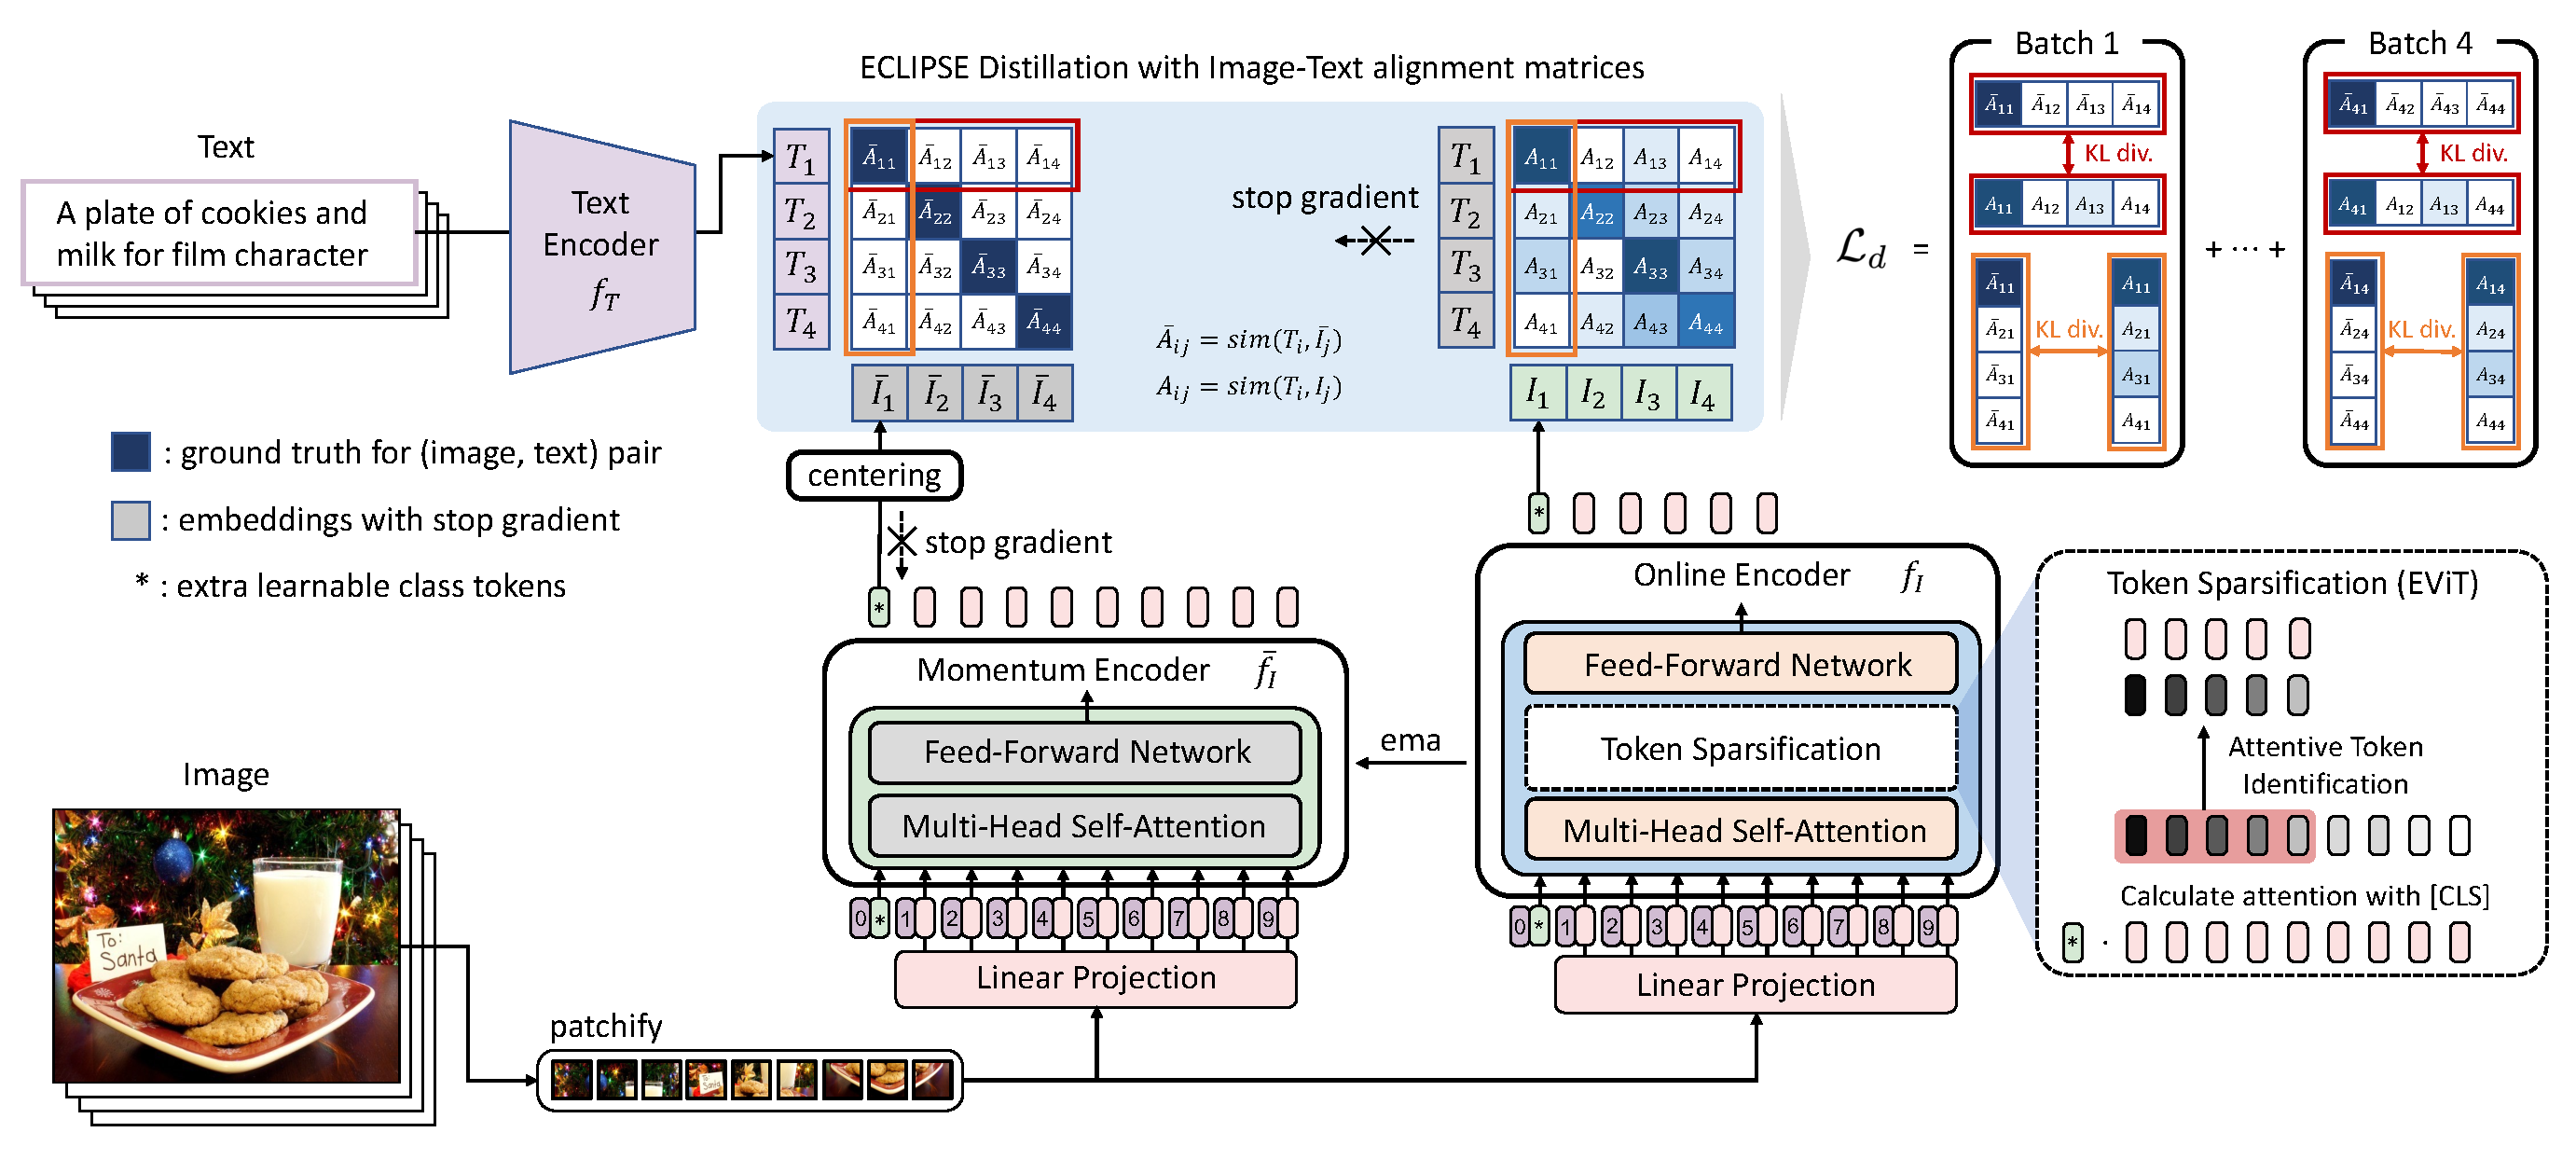
\includegraphics[width=0.9\textwidth]{figures/imgs/figure_overall.pdf}
    \caption{Overview of our proposed ECLIPSE. ECLIPSE is a meta-architecture for contrastive language-image pretraining that features a text encoder $f_T$, a momentum teacher encoder (Full ViT, $\bar{f}_I$), and a streamlined online encoder (ViT with token sparsification, $f_I$). Though the online network of ECLIPSE is compatible with any ViT acceleration method in literature~\cite{liang2022evit,rao2021dynamicvit,liang2022expediting}, we choose EViT~\cite{liang2022evit} due to its simple architecture without introducing additional parameters. Full ViTs without any sparsification can be also adopted for the online network, in which ECLIPSE then provides a full-capacity model with enhanced performance.
    }
    \label{fig:fig_architecture}
\end{figure*}